\part{Polymorphism}
\frame{\partpage}

\begin{frame}{Polymorphism}
\begin{itemize}
	\pause\item From Greek: ``many-shape-ism''
	\pause\item Different classes can have the \textbf{same public interface}
	\pause\item Thus we can write code that \textbf{uses} this interface, but doesn't need to worry about the \textbf{implementation} behind it
\end{itemize}
\end{frame}

\begin{frame}{Method overriding}
\begin{itemize}
	\pause\item A class can \textbf{override} methods defined in the class from which it inherits
	\pause\item The overridden method can call the method from the base class, but it doesn't have to
\end{itemize}
\end{frame}

\begin{frame}[fragile]{Without polymorphism}
	\begin{lstlisting}
class Shape { ... };
class Circle : public Shape { ... };
class Square : public Shape { ... };
class Triangle : public Shape { ... };

std::vector<Shape*> shapes;
// Populate shapes with circles, squares, triangles...

for (Shape* shape : shapes)
{
	if (shape->isCircle)
		drawCircle(shape->centre, shape->radius);
	else if (shape->isSquare)
		drawSquare(shape->centre, shape->size);
	...
}
	\end{lstlisting}
\end{frame}

\begin{frame}[fragile]{Polymorphism to the rescue!}
	\begin{lstlisting}
class Shape {
	public: virtual void draw() {}
};
class Circle : public Shape {
	public: void draw() override {
		drawCircle(centre, radius);
	}
};
class Square : public Shape {
	public: void draw() override {
		drawSquare(centre, size);
	}
};

for (Shape* shape : shapes)
	shape->draw();
	\end{lstlisting}
\end{frame}

\begin{frame}{Polymorphism to the rescue!}
	\begin{itemize}
		\pause\item All subclasses of \lstinline{Shape} implement \lstinline{draw}
		\pause\item We can call \lstinline{shape->draw()} without worrying which type of shape it is
		\pause\item The \textbf{virtual method table} takes care of calling the correct
			\lstinline{draw} function depending on the type of \lstinline{shape},
			no extra code required
	\end{itemize}
\end{frame}

\begin{frame}[fragile]{Instance types}
	\pause
	\begin{lstlisting}
Shape myShape;
	\end{lstlisting}
	\begin{itemize}
		\pause\item \lstinline{myShape} is an instance of \lstinline{Shape}, allocated on the \textbf{stack}
	\end{itemize}
	\pause
	\begin{lstlisting}
Shape* myShapePtr;
	\end{lstlisting}
	\begin{itemize}
		\pause\item \lstinline{myShapePtr} points to an instance of \lstinline{Shape}
			or of a subclass of \lstinline{Shape}, allocated on the \textbf{heap}
		\pause\item Polymorphism works for pointers, but not for instances on the stack
	\end{itemize}
\end{frame}

\begin{frame}{Abstract classes}
\begin{itemize}
	\pause\item Some classes should never be instantiated directly, as they only exist to be inherited from
	\begin{itemize}
		\pause\item \lstinline{Shape} is an example
	\end{itemize}
	\pause\item Such classes are called \textbf{abstract}
	\pause\item Abstract classes generally have one or more \textbf{pure virtual methods} ---
		methods which are left unimplemented so \textbf{must} be implemented in subclasses
\end{itemize}
\end{frame}

\begin{frame}[fragile]{Abstract class example}
	\begin{lstlisting}
class Shape
{
public:
	virtual void draw() = 0;
};
	\end{lstlisting}
	\begin{itemize}
		\pause\item Here \lstinline{= 0} marks the method as \textbf{pure virtual}
		\pause\item In C++, having at least one pure virtual method implicitly marks the class as \textbf{abstract}
		\pause\item Now you will get a compile error if you try to instantiate \lstinline{Shape} directly
		\pause\item To become not abstract, subclasses of \lstinline{Shape} must override \lstinline{draw}
		\pause\item Subclasses of \lstinline{Shape} which \textbf{do} override \lstinline{draw} can be instantiated
		\pause\item Trying to instantiate a subclass of \lstinline{Shape} which \textbf{does not} override \lstinline{draw}
			will also give a compile error
	\end{itemize}
\end{frame}

\begin{frame}[fragile]{Interfaces}
	\begin{itemize}
		\pause\item An abstract class in which \textbf{all} methods are pure virtual is called an \textbf{interface}
		\pause\item Interfaces do not contain any implementation, but specify a set of methods which subclasses
			must implement
		\pause\item NB: some languages (e.g.\ C\#, Java) make a distinction between classes and interfaces;
			C++ does not
	\end{itemize}
\end{frame}

\begin{frame}{OOP design}
	\begin{center}
		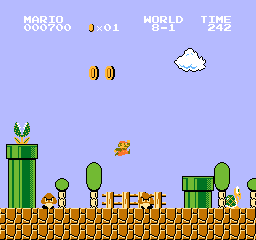
\includegraphics[height=0.4\textheight]{mario}
		\hspace{0.1\textwidth}
		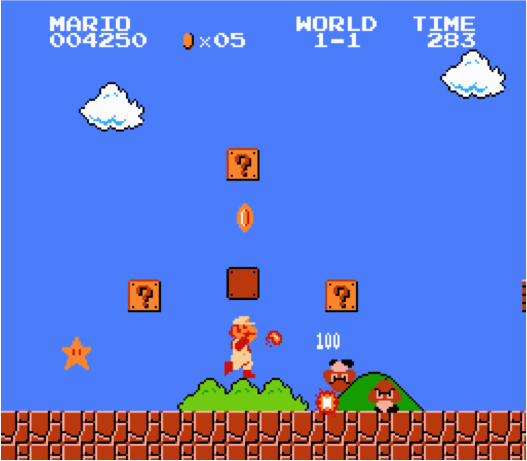
\includegraphics[height=0.4\textheight]{mario2}
	\end{center}
	\begin{itemize}
		\item What \textbf{classes} might be defined in a Mario-style platform game?
		\item What classes might \textbf{inherit} from one another?
	\end{itemize}
\end{frame}
